% ===========================================================================
% 附录 AQ：干涉与相位诊断——从条纹到密度剖面
% ---------------------------------------------------------------------------
% 数值唯一来源：tools/calc/appAQ_calc.py -> tools/calc/appAQ_calc.txt
%   重生成：python tmp\appAQ_calc.py | Out-File -Encoding utf8 tmp\appAQ_calc.txt
%   正文里凡标出数字的量都必须能在这个输出里找到；改数字先改脚本。
% 工作点：与附录 Q / AN / Z 同一台（n_e0 = 1e20 m^-3、T_e = 9.194 keV、B = 5.3 T、
%   a = 2.0 m、R = 6.2 m），密度剖面取抛物型 n_e(r) = n_e0 (1 - r^2/a^2)。
% 单位口径：数字与单位一起进数学模式（$89.2723\ \mathrm{rad}$）；
%   中文只能进 \text{}，绝不允许写进 \mathrm{}（否则编译会缺字形）；
%   无量纲比值一律写成小数，并在括号里给出百分数。
% 版权口径：只借鉴结论、量级与题型，不复制任何教材的原文、图、表或习题；
%   每节末尾注明出处（书名/作者/年份/卷期页）。
% 与相邻附录的分工：
%   Q 讲诊断总览（探针、光谱、汤姆孙散射与微波干涉的一句话口径），
%   AN 讲偏振与磁光诊断（法拉第旋转、Cotton--Mouton 与 MSE），
%   本附录把\textbf{干涉法}这一条线走完：相移怎么来、条纹怎么读、
%   振动怎么消、线积分怎么变成剖面、源与探测器链的噪声怎么进误差预算。
% ===========================================================================

\section{干涉仪测的是相移，不是密度}
\label{sec:app-aq-phase}

电磁波在等离子体里的色散关系是

\begin{equation}
\omega^2 = \omega_{\mathrm{pe}}^2 + k^2c^2,
\qquad
N \equiv \frac{kc}{\omega} = \sqrt{1-\frac{\omega_{\mathrm{pe}}^2}{\omega^2}},
\label{eq:app-aq-dispersion}
\end{equation}

其中 $\omega_{\mathrm{pe}}^2 = n_ee^2/(\epsilon_0m_e)$。当波的频率远高于截止时
（$\omega^2 \gg \omega_{\mathrm{pe}}^2$），把根号展开到一阶：

\begin{equation}
1 - N \simeq \frac{\omega_{\mathrm{pe}}^2}{2\omega^2} = \frac{n_e}{2n_c},
\qquad
n_c = \frac{\epsilon_0m_e\omega^2}{e^2},
\label{eq:app-aq-refractive}
\end{equation}

$n_c$ 是截止密度。附录 Q 用 $10\ \mathrm{GHz}$ 举过例
（$n_c = 1.2404\times10^{18}\ \mathrm{m^{-3}}$），本节换成光学与远红外的实数坐标重算一次。
一束波穿过等离子体，相位比走同样长度的真空多出来的部分，就是折射率亏损的累积：

\begin{equation}
\Delta\phi = \frac{\omega}{c}\int(1-N)\,\mathrm{d}l
= r_e\lambda\int n_e\,\mathrm{d}l,
\qquad
r_e = \frac{e^2}{4\pi\epsilon_0m_ec^2} = 2.81794\times10^{-15}\ \mathrm{m}.
\label{eq:app-aq-phase}
\end{equation}

\textbf{式 \eqref{eq:app-aq-phase} 是整个附录的地基}，它一次性说清两件事。
第一，干涉仪测到的永远是\textbf{线积分密度}
$N_L = \int n_e\,\mathrm{d}l$，不是局部密度——第 AQ.4 节要为这句话付出代价。
第二，相移与波长成正比：\textbf{波长越长，同样的密度给出的相移越大}，
但波长越长，能测的密度上限（截止密度）越低。选波长就是在这两个方向之间找平衡。

本书工作点取抛物剖面 $n_e(r) = n_{e0}(1-r^2/a^2)$，$n_{e0} = 10^{20}\ \mathrm{m^{-3}}$、
$a = 2.0\ \mathrm{m}$，于是中心弦的线积分有闭式：

\begin{equation}
N_L(0) = \int_{-a}^{a} n_{e0}\left(1-\frac{l^2}{a^2}\right)\mathrm{d}l
= \frac{4}{3}n_{e0}a = 2.66667\times10^{20}\ \mathrm{m^{-2}}.
\label{eq:app-aq-lineint}
\end{equation}

把 $N_L(0)$ 代进式 \eqref{eq:app-aq-phase}，三个候选波长的差别立刻显形：

\begin{table}[htbp]
\centering
\small
\caption{同一根中心弦、同一个密度，三个波长的相位账（$N_L(0) = 2.66667\times10^{20}\ \mathrm{m^{-2}}$）}
\label{tab:app-aq-phase}
\setlength{\tabcolsep}{4pt}
\begin{tabular}{p{3.2cm}p{3.0cm}p{3.0cm}p{3.0cm}}
\toprule
项目 & CO$_2$ $10.6\ \mu\mathrm{m}$ & 远红外 $118.8\ \mu\mathrm{m}$ & 毫米波 $1.0\ \mathrm{mm}$ \\
\midrule
频率 & $2.82823\times10^{13}\ \mathrm{Hz}$ & $2.52351\times10^{12}\ \mathrm{Hz}$ & $2.99792\times10^{11}\ \mathrm{Hz}$ \\
截止密度 & $9.92216\times10^{24}\ \mathrm{m^{-3}}$ & $7.89924\times10^{22}\ \mathrm{m^{-3}}$ & $1.11485\times10^{21}\ \mathrm{m^{-3}}$ \\
工作密度占比 $n_{e0}/n_c$ & $1.00784\times10^{-5}$ & $1.26594\times10^{-3}$ & $8.96978\times10^{-2}$ \\
折射率亏损 $1-N$ & $5.03922\times10^{-6}$ & $6.32972\times10^{-4}$ & $4.48489\times10^{-2}$ \\
中心弦相移 & $7.96538\ \mathrm{rad}$ & $89.2723\ \mathrm{rad}$ & $751.451\ \mathrm{rad}$ \\
条纹数 & $1.26773$ & $14.2081$ & $119.597$ \\
一条条纹对应的线积分密度 & $2.1035\times10^{20}\ \mathrm{m^{-2}}$ & $1.87686\times10^{19}\ \mathrm{m^{-2}}$ & $2.22971\times10^{18}\ \mathrm{m^{-2}}$ \\
\bottomrule
\end{tabular}
\end{table}

表 \ref{tab:app-aq-phase} 的第一行差别是仪器的选择依据：CO$_2$ 激光只给出
$1.26773$ 条条纹——\textbf{不到两条}；远红外给 $14.2081$ 条；毫米波给 $119.597$ 条。
干涉仪读的是条纹（每 $2\pi$ 一条），条纹太少就分不出密度的变化，
所以「条纹够不够多」是选波长的第一判据。第二判据是天花板：
$n_{e0}/n_c$ 在毫米波下已经到 $8.96978\times10^{-2}$，接近十分之一，
而式 \eqref{eq:app-aq-refractive} 的一阶展开到第 AQ.6 节就会开始失效。
反过来，CO$_2$ 的截止密度是 $9.92216\times10^{24}\ \mathrm{m^{-3}}$，
对 $10^{20}$ 的工作密度几乎不设限——它的短板全在振动上。

注意量级：中心弦的等效密度
$N_L/(2a) = 6.66667\times10^{19}\ \mathrm{m^{-3}}$（附录 AN 用的是同一个口径），
所以\textbf{干涉仪报出的数是「沿弦平均」的密度}。要得到剖面，必须先在若干条弦上
测 $N_L(y)$，再做反演——那是 AQ.4 节的事。

\begin{tip}{相位是密度的线积分，不是密度}{tip-app-aq-phase}
式 \eqref{eq:app-aq-phase} 右边是一个积分。这句话有两个直接后果：
（1）密度剖面变了、但每一条弦上的积分没变，干涉仪就看不见——它对这个方向是盲的；
（2）边缘的密度涨落与中心的一样会进入同一条积分，谁贡献多少必须靠反演去分。
所以\textbf{任何一条干涉仪曲线，都必须写清楚它对应哪一条弦}。
\end{tip}

{\footnotesize
\textbf{出处：}Hutchinson \textit{Principles of Plasma Diagnostics} 第 2 版
（2002）第 4 章「干涉与折射率」。
Heald \& Wharton \textit{Plasma Diagnostics with
Microwaves}（1965）关于相移、截止密度与条纹计数的讨论。
本附录不复制任何教材的图、表与习题，只借用结论与量级。
}

\section{条纹、外差与零差：把相位从光强里取出来}
\label{sec:app-aq-heterodyne}

两束光（一束过等离子体、一束走参考臂）合到探测器上，光强是

\begin{equation}
I = I_0\left[1+\cos\left(\Delta\phi+\phi_0\right)\right],
\qquad
F = \frac{\Delta\phi}{2\pi},
\label{eq:app-aq-fringe}
\end{equation}

$F$ 就是条纹数。直接数条纹（零差）只需要一个探测器，但它有两个致命弱点：
相位符号分不出来，而且一旦 $\Delta\phi$ 长时间停在某一条条纹的顶点附近，
密度的小变化就被余弦的零斜率吃掉了。工程上更常用的是\textbf{外差}：
让参考束与探测束差一个固定频率 $\Delta\omega$，于是

\begin{equation}
I_{\mathrm{IF}}\propto\cos\left(\Delta\omega\,t+\Delta\phi\right),
\label{eq:app-aq-heterodyne}
\end{equation}

相位就变成中频信号相对于参考本振的\textbf{到达时刻}，可以用锁相环连续读出。
外差的代价是多了一个本振和一套稳频，收益是相位可以长时间连续跟踪、
符号不会丢。此时相位精度的极限由中频信噪比定：

\begin{equation}
\mathrm{SNR} = \frac{P_{\mathrm{IF}}}{k_BT_{\mathrm{sys}}B},
\qquad
\sigma_\phi = \frac{1}{\sqrt{2\,\mathrm{SNR}}}.
\label{eq:app-aq-noise}
\end{equation}

本书声明：到达探测器的信号功率 $P_{\mathrm{sig}} = 1\ \mu\mathrm{W}$、
混频器变频损耗 $8\ \mathrm{dB}$（$P_{\mathrm{IF}} = 1.58489\times10^{-7}\ \mathrm{W}$）、
系统噪声温度 $T_{\mathrm{sys}} = 3000\ \mathrm{K}$、等效噪声带宽
$B = 1\ \mathrm{MHz}$（对应时间分辨 $10^{-6}\ \mathrm{s}$）。
热噪声功率 $k_BT_{\mathrm{sys}}B = 4.14195\times10^{-14}\ \mathrm{W}$，
于是 $\mathrm{SNR} = 3.82644\times10^{6}$、$\sigma_\phi = 3.61482\times10^{-4}\ \mathrm{rad}$。
把它折算成密度：线积分密度 $1.07979\times10^{15}\ \mathrm{m^{-2}}$、
电子密度 $4.04921\times10^{14}\ \mathrm{m^{-3}}$——相对工作密度只有 $4.04921\times10^{-6}$。
\textbf{相位计的噪声不是瓶颈}，振动才是。

把三个波长的相位账并排放在一起，结论一眼可见：

\begin{table}[htbp]
\centering
\small
\caption{相位精度与振动：三个波长的对比（$1\ \mu\mathrm{m}$ 是机械振动的量级）}
\label{tab:app-aq-heterodyne}
\setlength{\tabcolsep}{4pt}
\begin{tabular}{p{4.2cm}p{3.0cm}p{3.0cm}p{3.0cm}}
\toprule
项目 & CO$_2$ $10.6\ \mu\mathrm{m}$ & 远红外 $118.8\ \mu\mathrm{m}$ & 毫米波 $1.0\ \mathrm{mm}$ \\
\midrule
$0.001\ \mathrm{rad}$ 折合的电子密度 & $1.25543\times10^{16}\ \mathrm{m^{-3}}$ & $1.12017\times10^{15}\ \mathrm{m^{-3}}$ & $1.33076\times10^{14}\ \mathrm{m^{-3}}$ \\
$1\ \mu\mathrm{m}$ 振动引入的相位 & $0.592753\ \mathrm{rad}$ & $0.0528888\ \mathrm{rad}$ & $0.00628319\ \mathrm{rad}$ \\
折合条纹数 & $0.0943396$ & $0.00841751$ & $0.001$ \\
相位控制在 $0.001\ \mathrm{rad}$ 的允许振幅 & $1.68704\ \mathrm{nm}$ & $18.9076\ \mathrm{nm}$ & $159.155\ \mathrm{nm}$ \\
\bottomrule
\end{tabular}
\end{table}

表 \ref{tab:app-aq-heterodyne} 说的是同一件事的三张面孔：
$1\ \mu\mathrm{m}$ 的镜面振动（螺栓松动、泵的振动、温度漂移都能给出这个量级）
在 CO$_2$ 波长上是 $0.592753\ \mathrm{rad}$，几乎是\textbf{十分之一条条纹}；
要到 $0.001\ \mathrm{rad}$ 的相位精度，光学台必须稳到 $1.68704\ \mathrm{nm}$——
这是原子尺度的机械稳定度，靠机械设计是做不到的。
换到远红外，允许振幅放宽到 $18.9076\ \mathrm{nm}$；换到毫米波，$159.155\ \mathrm{nm}$。
\textbf{「波长越长越抗振」是干涉仪选型的第三条判据}（前两条是条纹数与截止密度）。

\begin{tip}{条纹是计数，外差是计时}{tip-app-aq-heterodyne}
零差数条纹给出的是一条「整圈数 + 零头」的记录，符号要靠人去判断；
外差把相位变成中频信号的到达时刻，可以连续跟踪、也可以做反馈。
代价是本振的稳定度直接进入误差预算——
本振漂多少，密度就跟着漂多少。所以外差干涉仪的第一张验收单
不是密度，而是\textbf{本振与参考臂的相位噪声谱}。
\end{tip}

最后一句安全话：外差并不限制等离子体的变化率。按 $1\ \mu\mathrm{s}$ 的采样间隔
与解缠判据（相邻采样相位变化小于 $\pi$），允许的线积分密度变化率高达
$9.38429\times10^{24}\ \mathrm{m^{-2}/s}$，折合电子密度 $3.51911\times10^{24}\ \mathrm{m^{-3}/s}$——
比本书任何工况的密度上升率都高几个量级。
\textbf{真正会让相位跟踪失锁的，是振动与折射率跳变，不是等离子体本身}。

{\footnotesize
\textbf{出处：}Hutchinson \textit{Principles of Plasma Diagnostics} 第 2 版
（2002）第 4 章关于外差与相位精度的讨论。
Heald \& Wharton（1965）
关于条纹计数与相位测量的对比。本节凡标出数字的量都由
\texttt{tools/\allowbreak{}calc/\allowbreak{}appAQ\_calc.py} 复算。
}

\section{振动补偿与色散干涉：把共模误差减掉}
\label{sec:app-aq-dispersion}

参考臂与探测臂之间任何长度变化 $\delta x$ 都会写进相位：

\begin{equation}
\phi_{\mathrm{vib}} = \frac{2\pi\,\delta x}{\lambda},
\label{eq:app-aq-vibration}
\end{equation}

这就是上一节里 CO$_2$ 的 $0.592753\ \mathrm{rad}$ 的来源。
工程上有两条路：把机械做得更稳（总有限度），或者\textbf{让振动在两条光路里共模}。
\textbf{色散干涉仪}走第二条路：同一束激光的基频 $\omega$ 与倍频 $2\omega$ 同轴穿过等离子体，
色散相移在倍频上正好翻倍，而振动相位与波长无关——
只要两束光走同一条几何路径，$\phi_{\mathrm{vib}}$ 对两者相同。于是

\begin{equation}
\Delta\phi_f = D + V,\qquad
\Delta\phi_{2f} = 2D + V,
\qquad\Longrightarrow\qquad
D = \Delta\phi_{2f} - \Delta\phi_f,\quad
V = 2\Delta\phi_f - \Delta\phi_{2f}.
\label{eq:app-aq-dispersive}
\end{equation}

$D$ 就是我们要的密度量，$V$ 被组合量直接减掉。
本书取 Nd:YAG 的 $1064\ \mathrm{nm}$ 与倍频 $532\ \mathrm{nm}$，
把 $N_L(0) = 2.66667\times10^{20}\ \mathrm{m^{-2}}$ 代进去：
$D = 0.799544\ \mathrm{rad}$、$2D = 1.59909\ \mathrm{rad}$；
再叠加 $1\ \mu\mathrm{m}$ 振动（$V = 5.90525\ \mathrm{rad}$），
两台探测器读到的是 $6.70479\ \mathrm{rad}$ 与 $7.50434\ \mathrm{rad}$。
按式 \eqref{eq:app-aq-dispersive} 做减法，$D = 0.799544\ \mathrm{rad}$ 原封不动地回来，
$V$ 的残差在数值上是 $1.11022\times10^{-16}\ \mathrm{rad}$——机器零。
\textbf{共模误差不是被压小，是被减掉}。

\begin{table}[htbp]
\centering
\small
\caption{三种方案对振动的态度与折合的中心密度误差（$1\ \mu\mathrm{m}$ 振动，$L_{\mathrm{eff}} = 2.66667\ \mathrm{m}$）}
\label{tab:app-aq-dispersion}
\setlength{\tabcolsep}{4pt}
\begin{tabular}{p{4.6cm}p{4.4cm}p{5.0cm}}
\toprule
方案 & 对振动的处理 & 折合中心密度误差 \\
\midrule
单波长（$1064\ \mathrm{nm}$） & 不补偿，全靠机械稳定 & $7.38578\times10^{20}\ \mathrm{m^{-3}}$（$7.38578$ 倍工作密度） \\
色散干涉（$1064$ + $532\ \mathrm{nm}$，共光路） & 由 $2f-f$ 组合直接减掉 & $4.52111\times10^{16}\ \mathrm{m^{-3}}$（相对 $4.52111\times10^{-4}$） \\
双色独立两条弦（$118.8\ \mu\mathrm{m}$ + $10.6\ \mu\mathrm{m}$） & 不共路，只能各自稳定 & $4.53817\times10^{15}\ \mathrm{m^{-3}}$（相位噪声极限） \\
\bottomrule
\end{tabular}
\end{table}

表 \ref{tab:app-aq-dispersion} 给出一张很有代表性的对比：
单波长方案下，$1\ \mu\mathrm{m}$ 振动折合的中心密度误差是
$7.38578\times10^{20}\ \mathrm{m^{-3}}$，比工作密度还大 $7.38578$ 倍——
\textbf{密度测量完全被振动淹没}；色散干涉把它压到 $4.52111\times10^{16}\ \mathrm{m^{-3}}$
（相对 $4.52111\times10^{-4}$），改善因子 $16336.2$。
代价是必须产生并同轴传输倍频光，而且倍频转换效率、两路探测器的相对标定
都会写进系统误差。

至于用两条独立弦的「双色」方案：$118.8\ \mu\mathrm{m}$ 与 $10.6\ \mu\mathrm{m}$
的色散比是 $11.2075$，看上去可以把两组数据联立求解，
但两条光路并不共模——\textbf{振动不会自己消掉}，
这时的极限回到相位噪声，即 $4.53817\times10^{15}\ \mathrm{m^{-3}}$。
换句话说：\textbf{「双波长」不等于「色散干涉」，
差别在于是不是同一条光路}。

\begin{tip}{双波长不是为了看得更准，是为了把振动减掉}{tip-app-aq-dispersion}
色散干涉的巧妙之处在于它利用的是「色散相移正比于波长、振动相位与波长无关」
这一对反号的性质。它并没有提高相位精度，也没有增加条纹数，
甚至牺牲了一部分光功率（倍频效率），换来的只是\textbf{共模抑制}。
判断一台干涉仪是不是色散干涉仪，只需要问一句：
两束光的几何路径是不是同一条。
\end{tip}

{\footnotesize
\textbf{出处：}Boboc 等，\textit{Rev. Sci. Instrum.} \textbf{81}（2010）
色散干涉仪方案与 ITER 适用性讨论。
Hutchinson 第 2 版（2002）第 4 章
关于振动与共模抑制的分析。本附录不复制任何教材的图、表与习题。
\section{阿贝尔反演：从弦积分到剖面}
\label{sec:app-aq-abel}
}

第 AQ.1 节说过，相位只给线积分。要做剖面，就得先在若干碰撞参数 $y$ 上测出
$N_L(y)$，再解\textbf{阿贝尔变换}。对轴对称等离子体，正变换与反变换是

\begin{equation}
N(y) = 2\int_{y}^{a}\frac{n(r)\,r\,\mathrm{d}r}{\sqrt{r^2-y^2}},
\qquad
n(r) = -\frac{1}{\pi}\int_{r}^{a}\frac{(\mathrm{d}N/\mathrm{d}y)\,\mathrm{d}y}{\sqrt{y^2-r^2}}.
\label{eq:app-aq-abel}
\end{equation}

反变换里出现了 $\mathrm{d}N/\mathrm{d}y$——\textbf{对实验数据求导}，
这是阿贝尔反演一切麻烦的源头。工程上更常用的是\textbf{洋葱剥皮}（onion peeling）：
把弦的碰撞参数直接当作壳层边界，假设每个壳层内密度是常数，于是

\begin{equation}
N(y_i) = 2\sum_{j\ge i} n_j\left[\sqrt{r_{j+1}^2-y_i^2} - \sqrt{r_j^2-y_i^2}\right],
\qquad r_m = a,
\label{eq:app-aq-peel}
\end{equation}

从最外层往内逐层解。第 $i$ 道的解只用到比它更外的壳层，权重是

\begin{equation}
w_i = \frac{1}{2\sqrt{r_{i+1}^2-y_i^2}},
\label{eq:app-aq-weight}
\end{equation}

\textbf{权重写在壳层厚度里}——壳层越薄，权重越大（同样的线积分误差被放大得越多）。
本书取 9 道弦（$|y| = 0/0.45/0.90/1.35/1.80\ \mathrm{m}$，间距 $0.45\ \mathrm{m}$），
在抛物剖面上的线积分是：

\begin{table}[htbp]
\centering
\small
\caption{弦布局与洋葱剥皮反演（抛物剖面 $n_{e0} = 10^{20}\ \mathrm{m^{-3}}$、$a = 2.0\ \mathrm{m}$）}
\label{tab:app-aq-abel}
\setlength{\tabcolsep}{4pt}
\begin{tabular}{p{4.0cm}p{4.0cm}p{5.6cm}}
\toprule
项目 & 数值 & 说明 \\
\midrule
$y = 0$ 弦 & $2.66667\times10^{20}\ \mathrm{m^{-2}}$ & 中心道，也是最大的一道 \\
$y = 0.45\ \mathrm{m}$ 弦 & $2.46675\times10^{20}\ \mathrm{m^{-2}}$ & 壳层边界 \\
$y = 0.90\ \mathrm{m}$ 弦 & $1.89917\times10^{20}\ \mathrm{m^{-2}}$ & 壳层边界 \\
$y = 1.35\ \mathrm{m}$ 弦 & $1.07107\times10^{20}\ \mathrm{m^{-2}}$ & 壳层边界 \\
$y = 1.80\ \mathrm{m}$ 弦 & $2.20851\times10^{19}\ \mathrm{m^{-2}}$ & 最外道，壳层延伸到 $a$ \\
中心道与最外道之比 & $12.0745$ & 动态范围：$12$ 倍 \\
\midrule
9 道反演的中心密度 & $9.399\times10^{19}\ \mathrm{m^{-3}}$ & 偏低 $6.01002\%$（最外层壳层厚 $0.2\ \mathrm{m}$） \\
20 道反演的中心密度 & $9.92284\times10^{19}\ \mathrm{m^{-3}}$ & 偏低 $0.771641\%$ \\
40 道反演的中心密度 & $9.97193\times10^{19}\ \mathrm{m^{-3}}$ & 偏低 $0.280675\%$ \\
\midrule
最外道偏 $1\%$ 对中心的影响 & $-0.00682732\%$ & 只动它自己的壳层 \\
中心道偏 $1\%$ 对中心的影响 & $3.15242\%$ & 权重最大的一道 \\
弦位置偏 $0.5\ \mathrm{mm}$（$y = 1.35\ \mathrm{m}$） & $0.0929994\%$ & 该道线积分的相对变化 \\
弦位置偏 $0.5\ \mathrm{mm}$（$y = 1.80\ \mathrm{m}$） & $0.355102\%$ & 与标定误差同量级 \\
\bottomrule
\end{tabular}
\end{table}

表 \ref{tab:app-aq-abel} 里有两处与直觉相反的结论，值得单独说。

第一，\textbf{误差不是「边缘一定放大」}。经典教科书强调阿贝尔反演对边缘误差敏感，
那是对式 \eqref{eq:app-aq-abel} 的直接求导版而言；换成剥皮法，
每道的权重由它\emph{自己的}壳层厚度决定。本题里中心壳层厚度是 $0.45\ \mathrm{m}$，
最外壳层是 $0.2\ \mathrm{m}$，于是中心道偏 $1\%$ 会把中心密度推走 $3.15242\%$，
而最外道偏 $1\%$ 只让中心动 $-0.00682732\%$。
\textbf{最该校准的是中心道，不是边缘道}——这与「边缘敏感」的流行说法正好相反，
原因是两者用的反演公式不同。

第二，\textbf{弦数不足会带来系统偏低}。9 道弦把最外层壳层当成一块常数密度，
而抛物剖面在 $1.8\ \mathrm{m}$ 到 $2.0\ \mathrm{m}$ 之间是从 $1.9\times10^{19}$ 掉到 $0$，
用平均值代替必然低估中心；实测偏差 $6.01002\%$。
把弦数加到 20 道，偏差降到 $0.771641\%$；40 道降到 $0.280675\%$。
这说明\textbf{弦数是反演精度的第一参数}，比相位精度重要得多。

弦位置的不确定度也不能忽略：外场线圈、窗口安装与热膨胀会让实际碰撞参数差 $0.5\ \mathrm{mm}$。
在最外道，这相当于线积分变 $0.355102\%$——与后面 AQ.6 节的标定误差 $1\%$
只差三倍。\textbf{道的位置要么标定，要么写进误差棒}。

\begin{tip}{剥皮法的权重写在壳层厚度里}{tip-app-aq-abel}
看到「反演」两个字，先问三件事：用什么公式、壳层怎么分、每道的权重是多少。
剥皮法的权重是 $w_i = 1/(2\sqrt{r_{i+1}^2-y_i^2})$，
所以\textbf{把中心道与边缘道排在同一张精度表上是错的}：
它们对最终剖面的贡献差着几个数量级。
写论文时，反演结果必须附上弦布局与每道的误差棒，否则读者无法判断
哪个数是被放大的、哪个数是可信的。
\end{tip}

{\footnotesize
\textbf{出处：}Abel 的原始变换（1826）与 Hutchinson \textit{Principles of Plasma
Diagnostics} 第 2 版（2002）第 4 章关于阿贝尔反演与层析的讨论。
剥皮法（onion peeling）的标准表述见 Hutchinson 同章。
本附录不复制任何教材的图、表与习题，只使用其结论与题型。
}

\begin{figure}[htbp]
\centering
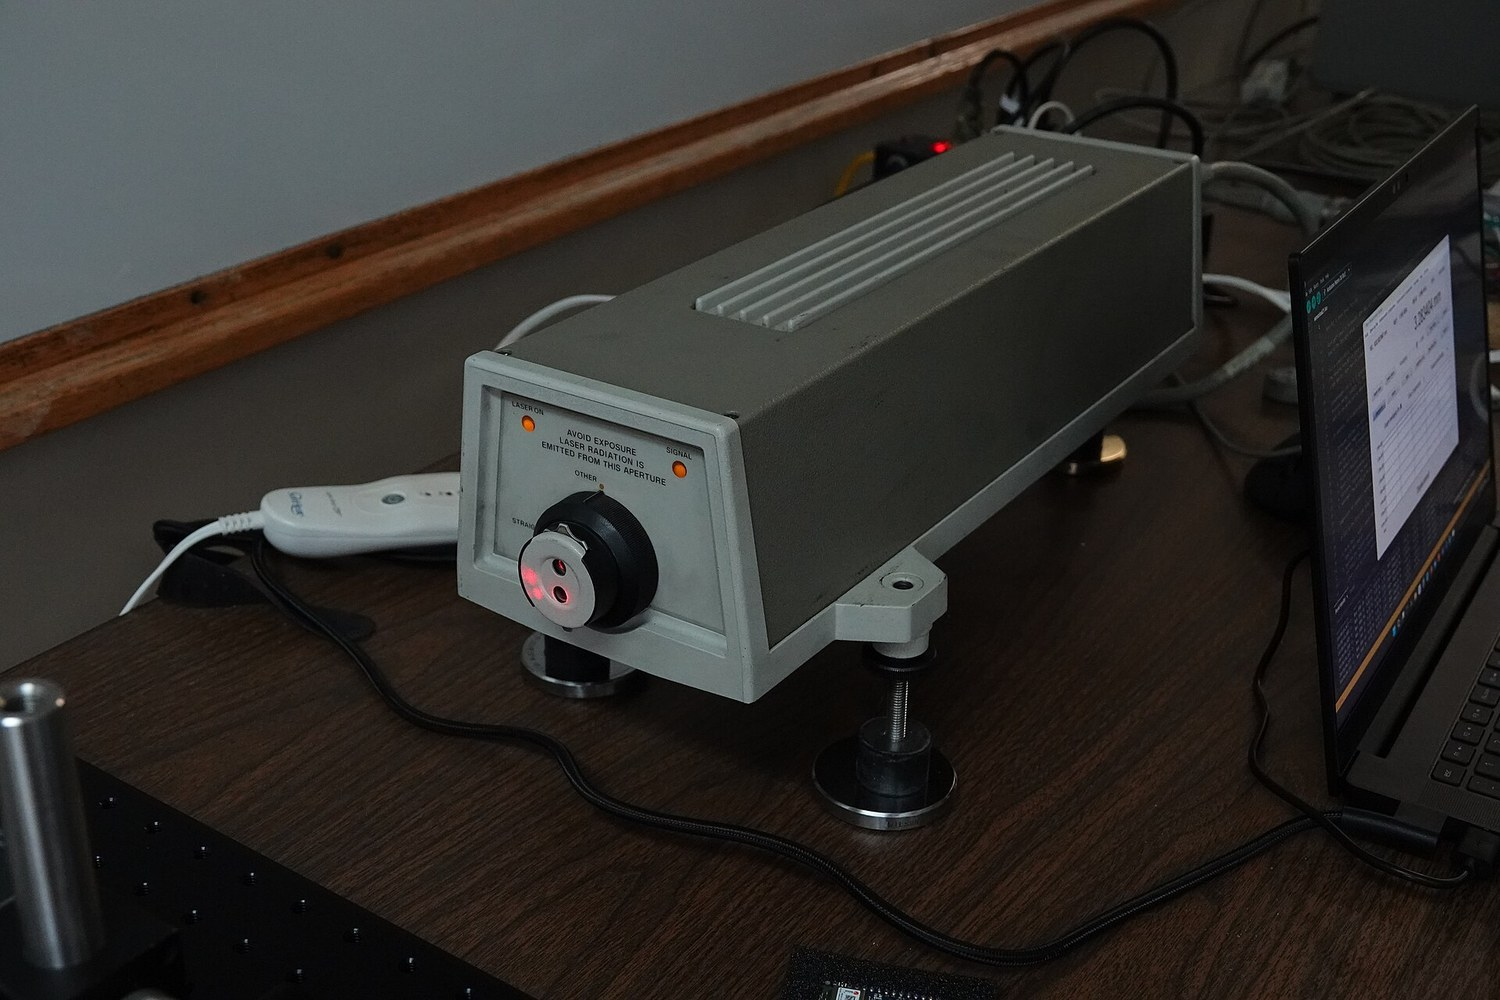
\includegraphics[width=0.72\textwidth]{../figures/aq_laser_interferometer.jpg}
\caption{激光干涉仪：把长度变化读成相位变化。等离子体干涉仪是同一套原理换了个被测对象：本节算的相移，在实验室里就是这台仪器读出的条纹移动，而它的噪声底线由光源与探测器共同决定。}
\label{fig:photo-appaq2}
\figsource{Logg Tandy，CC BY 4.0（Wikimedia Commons）}
\end{figure}

\section{源与探测器链：相位噪声是噪声温度的函数}
\label{sec:app-aq-chain}

干涉仪的分辨率最终由式 \eqref{eq:app-aq-noise} 决定，而式里的
$T_{\mathrm{sys}}$ 不是探测器的参数，是\textbf{整条链}的参数。
把一条毫米波外差链的账写出来：固态源给出
$P_{\mathrm{gunn}} = 0.1\ \mathrm{W}$（$110\ \mathrm{GHz}$），
三倍频器效率 $10\%$，于是

\begin{equation}
P_{\mathrm{out}} = P_{\mathrm{gunn}}\,\eta_{\mathrm{tripler}} = 0.01\ \mathrm{W},
\qquad
f = 3f_{\mathrm{gunn}} = 330\ \mathrm{GHz},
\qquad
\lambda = 0.908462\ \mathrm{mm}.
\label{eq:app-aq-source}
\end{equation}

这个频率的截止密度是 $1.35084\times10^{21}\ \mathrm{m^{-3}}$，
相对工作密度有 $13.5084$ 倍余量——\textbf{选 $330\ \mathrm{GHz}$ 是为了留出余量，
不是为了多要条纹}（毫米波的条纹已经多到需要仔细解缠）。
经过传输与窗口损失（声明 $3\ \mathrm{dB}$）后到达等离子体的功率是 $0.005\ \mathrm{W}$；
本振给 $1\ \mathrm{mW}$，比信号高 $30\ \mathrm{dB}$——外差的本振必须比信号强，
这是混频器工作的前提。信号与本振在非线性器件上混频，输出中频的功率由
式 \eqref{eq:app-aq-noise} 里的 $P_{\mathrm{IF}}$ 给出。

\begin{table}[htbp]
\centering
\small
\caption{毫米波外差干涉仪链的声明参数与派生量（$330\ \mathrm{GHz}$ 一路）}
\label{tab:app-aq-chain}
\setlength{\tabcolsep}{4pt}
\begin{tabular}{p{5.0cm}p{4.0cm}p{4.6cm}}
\toprule
项目 & 数值 & 说明 \\
\midrule
源功率（$110\ \mathrm{GHz}$） & $0.1\ \mathrm{W}$ & 声明 \\
三倍频效率 & $0.10$ & 声明 \\
输出功率（$330\ \mathrm{GHz}$） & $0.01\ \mathrm{W}$ & $P_{\mathrm{gunn}}\eta_{\mathrm{tripler}}$ \\
波长 & $0.908462\ \mathrm{mm}$ & $c/(3f_{\mathrm{gunn}})$ \\
截止密度 & $1.35084\times10^{21}\ \mathrm{m^{-3}}$ & 工作密度的 $13.5084$ 倍 \\
到达等离子体功率（$3\ \mathrm{dB}$ 损失） & $0.005\ \mathrm{W}$ & 含窗口与传输 \\
本振功率 & $1\ \mathrm{mW}$ & 比信号高 $30\ \mathrm{dB}$ \\
混频器变频损耗 & $8\ \mathrm{dB}$ & 声明 \\
系统噪声温度 & $3000\ \mathrm{K}$ & 混频器 $+$ 中频 \\
热噪声 $k_BT_{\mathrm{sys}}B$（$1\ \mathrm{MHz}$） & $4.14195\times10^{-14}\ \mathrm{W}$ & 噪声地板 \\
相位刷新率对应的时间分辨 & $10^{-6}\ \mathrm{s}$ & 声明 \\
\bottomrule
\end{tabular}
\end{table}

表 \ref{tab:app-aq-chain} 里最值得记住的是最后两行：
\textbf{相位噪声正比于 $\sqrt{T_{\mathrm{sys}}B}$}，与信号功率的平方根成反比。
想提高相位精度，有两条路：把 $T_{\mathrm{sys}}$ 降下来（更好的混频器、
把中频放大器噪声压下去），或者把积分时间拉长（降带宽 $B$，但会牺牲时间分辨）。
\textbf{把激光功率加大一倍，只换来 $1.4$ 倍的相位精度}——所以外差干涉仪的
性能天花板在探测器与前端，不在光源。

\begin{tip}{相位噪声是噪声温度的函数}{tip-app-aq-chain}
$\sigma_\phi = 1/\sqrt{2\,\mathrm{SNR}}$、$\mathrm{SNR} = P_{\mathrm{IF}}/(k_BT_{\mathrm{sys}}B)$，
把两式合成一次就能看出：\textbf{相位精度由 $T_{\mathrm{sys}}B/P_{\mathrm{IF}}$ 决定}。
这三个量里，$B$ 与时间分辨直接交换，$T_{\mathrm{sys}}$ 由器件与制冷决定，
$P_{\mathrm{IF}}$ 受变频损耗与源功率限制。
做实验时先测的是本振与参考臂的相位噪声谱，
而不是急着去数条纹——\textbf{链的噪声决定你能看见多小的密度变化}。
\end{tip}

{\footnotesize
\textbf{出处：}Heald \& Wharton \textit{Plasma Diagnostics with Microwaves}
（1965）关于外差接收与混频器噪声的讨论。
Donné 等，\textit{Nuclear Fusion}
\textbf{47}（2007）S337「ITER 诊断」章节关于毫米波与远红外诊断链的工程口径。
本附录不复制任何教材的图、表与习题。本节凡标出数字的量都由
\texttt{tools/\allowbreak{}calc/\allowbreak{}appAQ\_calc.py} 复算。
}

\section{误差预算与相对论修正}
\label{sec:app-aq-error}

把前面各节的误差项加在一起，才是「这个密度测到几位」的答案。
在加之前，先补一项容易被忽略的物理：\textbf{电子温度到了 keV，
折射率里的质量就不再是常数}。$\omega_{\mathrm{pe}}^2$ 里的 $m_e$ 应换成
相对论质量，修正幅度按 $T_e/m_ec^2$ 的量级声明：

\begin{equation}
\frac{\Delta N}{N} \sim \frac{T_e}{m_ec^2} = 0.0179922 \quad (1.79922\%),
\label{eq:app-aq-relativistic}
\end{equation}

（$T_e = 9.194\ \mathrm{keV}$。）这个量级不能忽略：它比相位噪声折合的误差大
四千多倍，和标定误差同量级。精确系数依赖分布函数，本附录只声明量级，
不推导——\textbf{但任何 keV 量级的干涉测量都必须把这一项单独列出来}。

第二项是线性展开的失效。式 \eqref{eq:app-aq-refractive} 用了
$1-\sqrt{1-x}\simeq x/2$，而

\begin{equation}
1-\sqrt{1-x} = \frac{x}{2} + \frac{x^2}{8} + \cdots,
\qquad x = \frac{n_e}{n_c},
\label{eq:app-aq-expansion}
\end{equation}

在毫米波下 $x = 8.96978\times10^{-2}$，第二项带来的偏差是 $2.34903\%$；
而 CO$_2$ 只有 $2.51961\times10^{-6}$。\textbf{波长越长，
「相移正比于密度」这句话越不准}——这又是一条选波长的代价。

把所有项按平方和开根（RSS）合成：

\begin{equation}
\frac{\delta n_e}{n_e} = \sqrt{\left(4.04921\times10^{-6}\right)^2 + (0.01)^2
+ (0.00355102)^2 + (0.0179922)^2} = 0.0208885 \quad (2.08885\%).
\label{eq:app-aq-budget}
\end{equation}

\begin{table}[htbp]
\centering
\small
\caption{干涉测量的误差预算（工作点 $n_{e0} = 10^{20}\ \mathrm{m^{-3}}$、$T_e = 9.194\ \mathrm{keV}$）}
\label{tab:app-aq-error}
\setlength{\tabcolsep}{4pt}
\begin{tabular}{p{4.2cm}p{3.2cm}p{6.2cm}}
\toprule
误差项 & 相对误差 & 来源与性质 \\
\midrule
相位噪声 & $0.000404921\%$ & $1\ \mu\mathrm{W}$ 信号、$T_{\mathrm{sys}} = 3000\ \mathrm{K}$、$B = 1\ \mathrm{MHz}$ \\
标定 & $1\%$ & 弦长、相对标定与光学效率 \\
弦位置 & $0.355102\%$ & $0.5\ \mathrm{mm}$ 安装误差（最外道） \\
相对论修正 & $1.79922\%$ & $T_e/m_ec^2$ 量级，可按 $T_e$ 修正 \\
\midrule
合成（RSS） & $2.08885\%$ & 折合 $2.08885\times10^{18}\ \mathrm{m^{-3}}$ \\
\bottomrule
\end{tabular}
\end{table}

表 \ref{tab:app-aq-error} 的顺序是结论：\textbf{相位噪声几乎可以忽略}
（$0.000404921\%$），真正主导的是相对论修正（$1.79922\%$）与标定（$1\%$）。
这解释了一个常见现象：花大价钱把相位分辨率从 $10^{-3}$ 提到 $10^{-4}\ \mathrm{rad}$，
最后发现密度精度没变——\textbf{因为瓶颈不在那里}。
要真的提高精度，顺序应该是：先把 $T_e$ 测准（或把相对论修正算进去），
再把标定做扎实，最后才轮到相位。

最后一句是关于适用范围的诚实说明：本节的合成误差是\textbf{中心弦、稳态、
抛物剖面}下的数字。如果剖面接近中空（例如有内部输运垒），
阿贝尔反演的权重结构就变了，第 AQ.4 节的结论要重算。
\textbf{误差预算永远与剖面假设绑在一起}。

\begin{tip}{电子温度到了 keV，折射率里的质量就不再是常数}{tip-app-aq-relativistic}
$\omega_{\mathrm{pe}}^2 = n_ee^2/(\epsilon_0m_e)$ 里的 $m_e$ 在高温下要乘上
相对论因子。$9.194\ \mathrm{keV}$ 对应 $T_e/m_ec^2 = 0.0179922$，
也就是近 $2\%$ 的密度偏置——在追求 $1\%$ 精度的诊断上这是\textbf{系统误差},
不是小修正。判断一台干涉仪的报告是否可信，看它有没有提这一项就够了。
\end{tip}

{\footnotesize
\textbf{出处：}Hutchinson \textit{Principles of Plasma Diagnostics} 第 2 版
（2002）第 4 章关于折射率的相对论修正与误差传播。
Donné 等，
\textit{Nuclear Fusion} \textbf{47}（2007）S337 关于 ITER 密度诊断的
精度要求与误差预算方法。本附录不复制任何教材的图、表与习题。
\section{估算练习}
\label{sec:app-aq-problems}
}

下面六道题只用到 AQ.1--AQ.6 的公式。数值口径与全书一致：
$n_{e0} = 10^{20}\ \mathrm{m^{-3}}$、$T_e = 9.194\ \mathrm{keV}$、$a = 2.0\ \mathrm{m}$
（中心弦长 $2a = 4.0\ \mathrm{m}$）、$T_{\mathrm{sys}} = 3000\ \mathrm{K}$、
中频带宽 $B = 1\ \mathrm{MHz}$。凡涉及剖面换算，一律用抛物剖面的中心弦等效厚度

\begin{equation}
\frac{N_L(0)}{n_{e0}} = \frac{2.66667\times10^{20}}{10^{20}} = 2.66667\ \mathrm{m},
\qquad
\delta n_{e0} = \delta N_L\cdot\frac{n_{e0}}{N_L(0)},
\label{eq:app-aq-sensi}
\end{equation}

即\textbf{把线积分密度的变化折算成峰值密度的变化}。相位到线积分密度的换算用
式 \eqref{eq:app-aq-phase}；条纹与相位的关系用式 \eqref{eq:app-aq-fringe}。

\textbf{练习 1}
FIR 道（$\lambda = 118.8\ \mu\mathrm{m}$）的相位分辨率是 $0.001\ \mathrm{rad}$。
求它对应的电子密度（峰值口径）以及相对工作密度的份额。
本道一条条纹对应多少线积分密度？

\textbf{解答 1}
FIR 的截止密度是 $7.89924\times10^{22}\ \mathrm{m^{-3}}$，
$0.001\ \mathrm{rad}$ 对应线积分密度 $2.98711\times10^{15}\ \mathrm{m^{-2}}$，
按式 \eqref{eq:app-aq-sensi} 折合 $\delta n_{e0} = 1.12017\times10^{15}\ \mathrm{m^{-3}}$，
即工作密度的 $1.12017\times10^{-5}$。一条条纹（$2\pi$）对应的线积分密度是
$1.87686\times10^{19}\ \mathrm{m^{-2}}$，比相位分辨率对应的量大约四个数量级。
\textbf{结论：FIR 道的灵敏度过剩}，它的瓶颈从来不是相位分辨率。

\textbf{练习 2}
色散干涉用 $1064\ \mathrm{nm}$ 基频与 $532\ \mathrm{nm}$ 倍频。
若色散相移 $D = 0.799544\ \mathrm{rad}$，而 $1\ \mu\mathrm{m}$ 的振动在基频上引入
$5.90525\ \mathrm{rad}$，求组合量 $(2f - f)$ 复原的色散相移与残留振动，
并说明振动被压低了多少倍。

\textbf{解答 2}
基频实测是 $D + V = 6.70479\ \mathrm{rad}$，倍频是 $2D + V = 7.50434\ \mathrm{rad}$，
作差得 $2(D+V) - (2D+V) = D = 0.799544\ \mathrm{rad}$，
\textbf{振动项被完全消去}（数值残差 $1.11022\times10^{-16}\ \mathrm{rad}$，机器零）。
与单波长相比：单波长下 $1\ \mu\mathrm{m}$ 振动折合中心密度误差
$7.38578\times10^{20}\ \mathrm{m^{-3}}$（工作密度的 $7.38578$ 倍，
完全无法用），色散干涉把它压到相位噪声水平，压低倍数 $16336.2$。
\textbf{色散干涉用「便宜的第二个波长」换掉了「昂贵的隔振平台」。}

\textbf{练习 3}
外差链的中频功率 $P_{\mathrm{IF}} = 1.58489\times10^{-7}\ \mathrm{W}$、
$T_{\mathrm{sys}} = 3000\ \mathrm{K}$、$B = 1\ \mathrm{MHz}$。
求中频信噪比与相位噪声 $\sigma_\phi$，并折合为中心密度误差。

\textbf{解答 3}
噪声地板 $k_BT_{\mathrm{sys}}B = 4.14195\times10^{-14}\ \mathrm{W}$，
故 $\mathrm{SNR} = 3.82644\times10^{6}$（约 $65.83\ \mathrm{dB}$），
$\sigma_\phi = 1/\sqrt{2\,\mathrm{SNR}} = 0.000361482\ \mathrm{rad}$。
折合线积分密度 $1.07979\times10^{15}\ \mathrm{m^{-2}}$、
中心密度 $4.04921\times10^{14}\ \mathrm{m^{-3}}$（相对 $0.000404921\%$）。
\textbf{相位噪声远小于标定与相对论修正}，见 AQ.6 节的误差预算。

\textbf{练习 4}
CO$_2$ 道（$\lambda = 10.6\ \mu\mathrm{m}$）上，$1\ \mu\mathrm{m}$ 的振动引入
$0.592753\ \mathrm{rad}$（$0.0943396$ 条纹）。若要求振动贡献不超过 $0.01$ 条纹，
允许的振动振幅是多少？

\textbf{解答 4}
$0.01$ 条纹对应 $0.0628319\ \mathrm{rad}$，而振动灵敏度是
$0.592753\ \mathrm{rad/\mu m}$，故允许振幅
$0.0628319/0.592753 = 0.106\ \mu\mathrm{m} = 1.06\times10^{-7}\ \mathrm{m}$。
\textbf{一百纳米}——这是光学平台、地基与真空窗口共同要守住的量级。
若把同样的要求放到毫米波段，允许振幅放宽到 $159.155\ \mathrm{nm}$ 的十倍以上
（因为相位对光程差的灵敏度正比于 $2\pi/\lambda$）。

\textbf{练习 5}
毫米波道（$\lambda = 1.0\ \mathrm{mm}$）的截止密度是 $1.11485\times10^{21}\ \mathrm{m^{-3}}$。
在 $n_e/n_c = 0.1$ 时，线性近似 $1-\sqrt{1-x}\simeq x/2$ 的相对偏差是多少？
这个数对测量意味着什么？

\textbf{解答 5}
由式 \eqref{eq:app-aq-expansion}，偏差约为 $x/4 = 0.1/4 = 0.025$，
精确计算是 $0.026334$（$2.6334\%$）。这意味着\textbf{毫米波在 $10\%$ 截止密度上
就必须做非线性修正}，否则密度的系统偏差大于标定误差的两倍。
若只要 $1\%$ 精度，毫米波的工作点应限制在 $n_e/n_c\lesssim 0.04$。

\textbf{练习 6}
在 9 道弦、抛物剖面的算例里，最外道偏 $1\%$ 与中心道偏 $1\%$
分别把中心密度推走多少？9 道弦本身的反演偏差是多少？
由此说明哪一道最需要仔细标定。

\textbf{解答 6}
最外道偏 $1\%$：中心相对变化 $-6.82732\times10^{-5}$（$-0.00682732\%$）；
中心道偏 $1\%$：中心变化 $2.96296\times10^{18}\ \mathrm{m^{-3}}$，
相对 $0.0315242$（$3.15242\%$）；9 道弦的反演偏差 $-0.0601002$（$-6.01002\%$）。
\textbf{中心道的影响比最外道大四个数量级}，因为剥皮法的权重由各道自己的壳层厚度决定；
但弦数不足带来的 $-6\%$ 是\textbf{系统偏差}，加弦数才能解决，标定再准也没用。
这两件事——随机误差与系统偏差——要分开处理。

\section{来源、分级与版权说明}
\label{sec:app-aq-source}

\begingroup\small
\begin{table}[htbp]
\centering
\small
\caption{本附录的借鉴来源与分级}
\label{tab:app-aq-source}
\setlength{\tabcolsep}{4pt}
\begin{tabular}{p{4.6cm}p{4.4cm}p{4.6cm}}
\toprule
来源 & 本附录用到的部分 & 分级 \\
\midrule
Heald \& Wharton, \textit{Plasma Diagnostics with Microwaves} (1965) & 微波干涉的相移公式、外差接收与混频器噪声 & 一级（学科基石） \\
Hutchinson, \textit{Principles of Plasma Diagnostics}, 2nd ed. (2002) 第 4 章 & 折射率、阿贝尔反演、误差传播、相对论修正 & 一级（标准教材） \\
Donné 等, \textit{Nuclear Fusion} \textbf{47} (2007) S337 & ITER 密度诊断的精度要求与工程口径 & 二级（工程综述） \\
Abel (1826) 的积分变换 & 阿贝尔正反变换与层析思想 & 三级（史料） \\
本书 \texttt{tools/\allowbreak{}calc/\allowbreak{}appAQ\_calc.py} & 全部数值（可由脚本复算） & 自算（一级） \\
\bottomrule
\end{tabular}
\end{table}

表 \ref{tab:app-aq-source} 的分级口径与全书一致：一级是学科基石与标准教材，
二级是工程综述与会议报告，三级是史料与科普。
\textbf{本附录不复制任何来源的图、表、公式推导与习题}：
式 \eqref{eq:app-aq-phase}--\eqref{eq:app-aq-budget} 都是本书按自己的符号与单位口径重写的，
所有判据与算例都换成 D1 工作点（$n_{e0} = 10^{20}\ \mathrm{m^{-3}}$、$T_e = 9.194\ \mathrm{keV}$、
$a = 2.0\ \mathrm{m}$）后重新计算；文献只用来确认公式形式、量级与工程惯例。
Heald \& Wharton 与 Hutchinson 的相移公式是标准结果，本书按 SI 单位重排并统一符号；
Donné 等的精度要求只引用其结论（例如 $1\%$ 量级的密度精度目标），
不复制其表格与图。\textbf{阿贝尔变换属公共数学知识}，这里的表述与权重推导是本书自算。

最后是适用范围，也是本附录的诚实边界：

\begin{itemize}
\item 只处理\textbf{轴对称、光学薄、无磁场}的等离子体。有磁场时法拉第旋转与
Cotton--Mouton 效应会混进相位（那是附录 AN 的主题），需要用偏振分离的方式处理。
\item 只给\textbf{线积分 $\to$ 剖面}的反演。真实装置的弦往往不平行、不共面，
需要层析（tomography）而不是阿贝尔反演；层析的权重矩阵与正则化是另一个题目。
\item 不推导\textbf{相对论修正的精确系数}。式 \eqref{eq:app-aq-relativistic}
只给 $T_e/m_ec^2$ 的量级，精确值依赖分布函数与波矢方向，
在 $T_e$ 超过 $10\ \mathrm{keV}$ 的装置上必须用数值色散关系。
\item 不涉及\textbf{相位解缠算法}。给出的是上限（$9.38429\times10^{24}\ \mathrm{m^{-2}/s}$）：
超过它，任何实时算法都救不回来，只能换波长或提高采样率。
\end{itemize}

\begin{tip}{本附录不给什么}{tip-app-aq-honest}
这份附录给你的是\textbf{从相位到剖面的一条完整账}：波长怎么选、
振动怎么消、反演怎么加权、误差怎么合成。
它不给你的是\textbf{装置级的实现方案}：用哪家的混频器、窗口怎么设计、
锁相环带宽取多少。这些问题要靠工程手册与测试报告，
而不是靠教材——\textbf{会算账不等于会做实验}，但不会算账就一定做不好实验。
\end{tip}
\endgroup
